\documentclass[a4paper,12pt]{article}

\usepackage{fontspec}
\usepackage{polyglossia}
\setdefaultlanguage{russian}
\setotherlanguage{english}
\setmainfont{DejaVu Serif}
\setsansfont{DejaVu Sans}
\setmonofont{DejaVu Sans Mono}

\usepackage{geometry}
\geometry{left=30mm,right=15mm,top=20mm,bottom=20mm}

\usepackage{graphicx}
\usepackage{float}
\usepackage{caption}
\usepackage{booktabs}
\usepackage{array}
\usepackage{enumitem}
\usepackage{hyperref}
\hypersetup{hidelinks}
\usepackage{xcolor}
\usepackage{fvextra}
\usepackage{tikz}
\usetikzlibrary{positioning,arrows.meta,fit,calc,backgrounds,shapes.geometric}

\setlength{\parindent}{1.25cm}
\setlength{\parskip}{0.25em}
\linespread{1.15}
\setlength{\emergencystretch}{3em}

\DefineVerbatimEnvironment{code}{Verbatim}{
    fontsize=\small,
    breaklines=true,
    breakanywhere=true,
    frame=single,
    framesep=3mm,
    rulecolor=\color{gray!45}
}

\newcommand{\placeholder}[1]{\textit{[заполнить: #1]}}

\begin{document}

\begin{titlepage}
\begin{center}
Федеральное государственное автономное образовательное учреждение\\
высшего образования\\
\textbf{«Национальный исследовательский университет ИТМО»}

\vfill

\textbf{\Large Лабораторная работа №1}\\[0.5em]
\textbf{\large по дисциплине «Информационные системы»}\\[1em]
Вариант № 11337

\vfill

\begin{flushright}
Выполнил:\\
Гришин Артем Евгеньевич\\
Р3311\\[1em]
Проверил:\\
Тюрин Иван Николаевич
\end{flushright}

\vfill

Санкт-Петербург\\
2026
\end{center}
\end{titlepage}

\tableofcontents
\newpage

\section{Задание}

Реализовать информационную систему, которая позволяет взаимодействовать с объектами класса
\texttt{Vehicle}, описание которого приведено ниже:

\begin{code}
public class Vehicle {
    private long id; // Значение поля должно быть больше 0,
                     // уникальным и генерироваться автоматически
    private String name; // Поле не может быть null, строка не может быть пустой
    private Coordinates coordinates; // Поле не может быть null
    private java.util.Date creationDate; // Поле не может быть null,
                                         // значение генерируется автоматически
    private VehicleType type; // Поле не может быть null
    private int enginePower; // Значение поля должно быть больше 0
    private int numberOfWheels; // Значение поля должно быть больше 0
    private long capacity; // Значение поля должно быть больше 0
    private Float distanceTravelled; // Поле может быть null,
                                     // значение должно быть больше 0
    private int fuelConsumption; // Значение поля должно быть больше 0
    private FuelType fuelType; // Поле не может быть null
}

public class Coordinates {
    private Double x; // Значение поля должно быть больше -415,
                      // поле не может быть null
    private Float y; // Максимальное значение поля: 663,
                     // поле не может быть null
}

public enum VehicleType {
    CAR,
    SUBMARINE,
    BICYCLE,
    HOVERBOARD;
}

public enum FuelType {
    ELECTRICITY,
    DIESEL,
    ANTIMATTER;
}
\end{code}

Разработанная система должна удовлетворять следующим требованиям:

\begin{itemize}[leftmargin=1.2cm]
    \item Основное назначение информационной системы --- управление объектами, созданными на основе заданного в варианте класса.
    \item Необходимо, чтобы с помощью системы можно было выполнить следующие операции с объектами: создание нового объекта, получение информации об объекте по ИД, обновление объекта (модификация его атрибутов), удаление объекта. Операции должны осуществляться в отдельных окнах (интерфейсах) приложения. При получении информации об объекте класса должна также выводиться информация о связанных с ним объектах.
    \item При создании объекта класса необходимо дать пользователю возможность связать новый объект с объектами вспомогательных классов, которые могут быть связаны с созданным объектом и уже есть в системе.
    \item Выполнение операций по управлению объектами должно осуществляться на серверной части (не на клиенте), изменения должны синхронизироваться с базой данных.
    \item На главном экране системы должен выводиться список текущих объектов в виде таблицы (каждый атрибут объекта --- отдельная колонка в таблице). При отображении таблицы должна использоваться пагинация, если все объекты не помещаются на одном экране.
    \item Нужно обеспечить возможность фильтровать/сортировать строки таблицы, которые показывают объекты, по значениям строковых колонок. Фильтрация элементов должна производиться по неполному совпадению.
    \item Переход к обновлению (модификации) объекта должен быть возможен из таблицы с общим списком объектов и из области с визуализацией объекта (при ее реализации).
    \item При добавлении/удалении/изменении объекта он должен автоматически появиться/исчезнуть/измениться в интерфейсах у других пользователей, авторизованных в системе.
    \item Если при удалении объекта с ним связан другой объект, связанные объекты должны быть связаны с другим объектом (по выбору пользователя), а изначальный объект удален.
    \item Пользователи должны иметь возможность просмотра всех объектов. Для модификации объекта должно открываться отдельное диалоговое окно. При вводе некорректных значений в поля объекта должны появляться информативные сообщения о соответствующих ошибках.
\end{itemize}

В системе должен быть реализован отдельный пользовательский интерфейс для выполнения специальных операций над объектами:

\begin{itemize}[leftmargin=1.2cm]
    \item Удалить все объекты, значение поля \texttt{fuelType} которого эквивалентно заданному.
    \item Вернуть один (любой) объект, значение поля \texttt{creationDate} которого является минимальным.
    \item Вернуть массив объектов, значение поля \texttt{fuelType} которых больше заданного.
    \item Найти все транспортные средства с мощностью двигателя в заданном диапазоне.
    \item Добавить транспортному средству с заданным id указанное число колёс.
    \item Представленные операции должны быть реализованы в рамках компонентов бизнес-логики приложения без прямого использования функций и процедур БД.
\end{itemize}

Особенности хранения объектов, которые должны быть реализованы в системе:

\begin{itemize}[leftmargin=1.2cm]
    \item Организовать хранение данных об объектах в реляционной СУБД (PostgreSQL). Каждый объект, с которым работает ИС, должен быть сохранён в базе данных.
    \item Все требования к полям класса (указанные в виде комментариев к описанию классов) должны быть выполнены на уровне ORM и БД.
    \item Для генерации поля id использовать средства базы данных.
    \item Для подключения к БД на кафедральном сервере использовать хост \texttt{pg}, имя базы данных \texttt{studs}, имя пользователя/пароль совпадают с таковыми для подключения к серверу.
\end{itemize}

При создании системы нужно учитывать следующие особенности организации взаимодействия с пользователем:

\begin{itemize}[leftmargin=1.2cm]
    \item Система должна реагировать на некорректный пользовательский ввод, ограничивая ввод недопустимых значений и информируя пользователей о причине ошибки.
    \item Переходы между различными логически обособленными частями системы должны осуществляться с помощью меню.
    \item При добавлении/удалении/изменении объекта он должен автоматически появиться/исчезнуть/измениться в области у всех других клиентов.
\end{itemize}

При разработке ИС должны учитываться следующие требования:

\begin{itemize}[leftmargin=1.2cm]
    \item В качестве основы для реализации ИС необходимо использовать Jakarta EE, CDI beans.
    \item Для создания уровня хранения необходимо использовать JPA + EclipseLink.
    \item Разные уровни приложения должны быть отделены друг от друга, разные логические части ИС должны находиться в отдельных компонентах.
\end{itemize}

\section{UML-диаграммы классов и пакетов}

\subsection{Диаграмма классов}

На диаграмме классов (рис.~\ref{fig:classes}) слои приложения идут сверху вниз: REST-ресурсы, сервисы, репозитории и сущности, а сбоку --- классы WebSocket. Сплошные стрелки означают, что класс хранит ссылку на другой класс (внедрён через \texttt{@Inject}), пунктирные --- зависимость: репозиторий работает с сущностью через JPQL, сервис отправляет CDI-событие, которое ловит \texttt{ChangeNotifier}.

Сверху показаны классы платформы Jakarta, к которым подключается приложение: \texttt{RestApplication} наследует \texttt{Application}, а три маппера реализуют \texttt{ExceptionMapper}, и каждый связан с исключением, которое он обрабатывает. Напрямую мапперы никто не вызывает: сервис бросает исключение, а JAX-RS сам находит подходящий \texttt{@Provider} по типу исключения.

\begin{figure}[p]
    \centering
    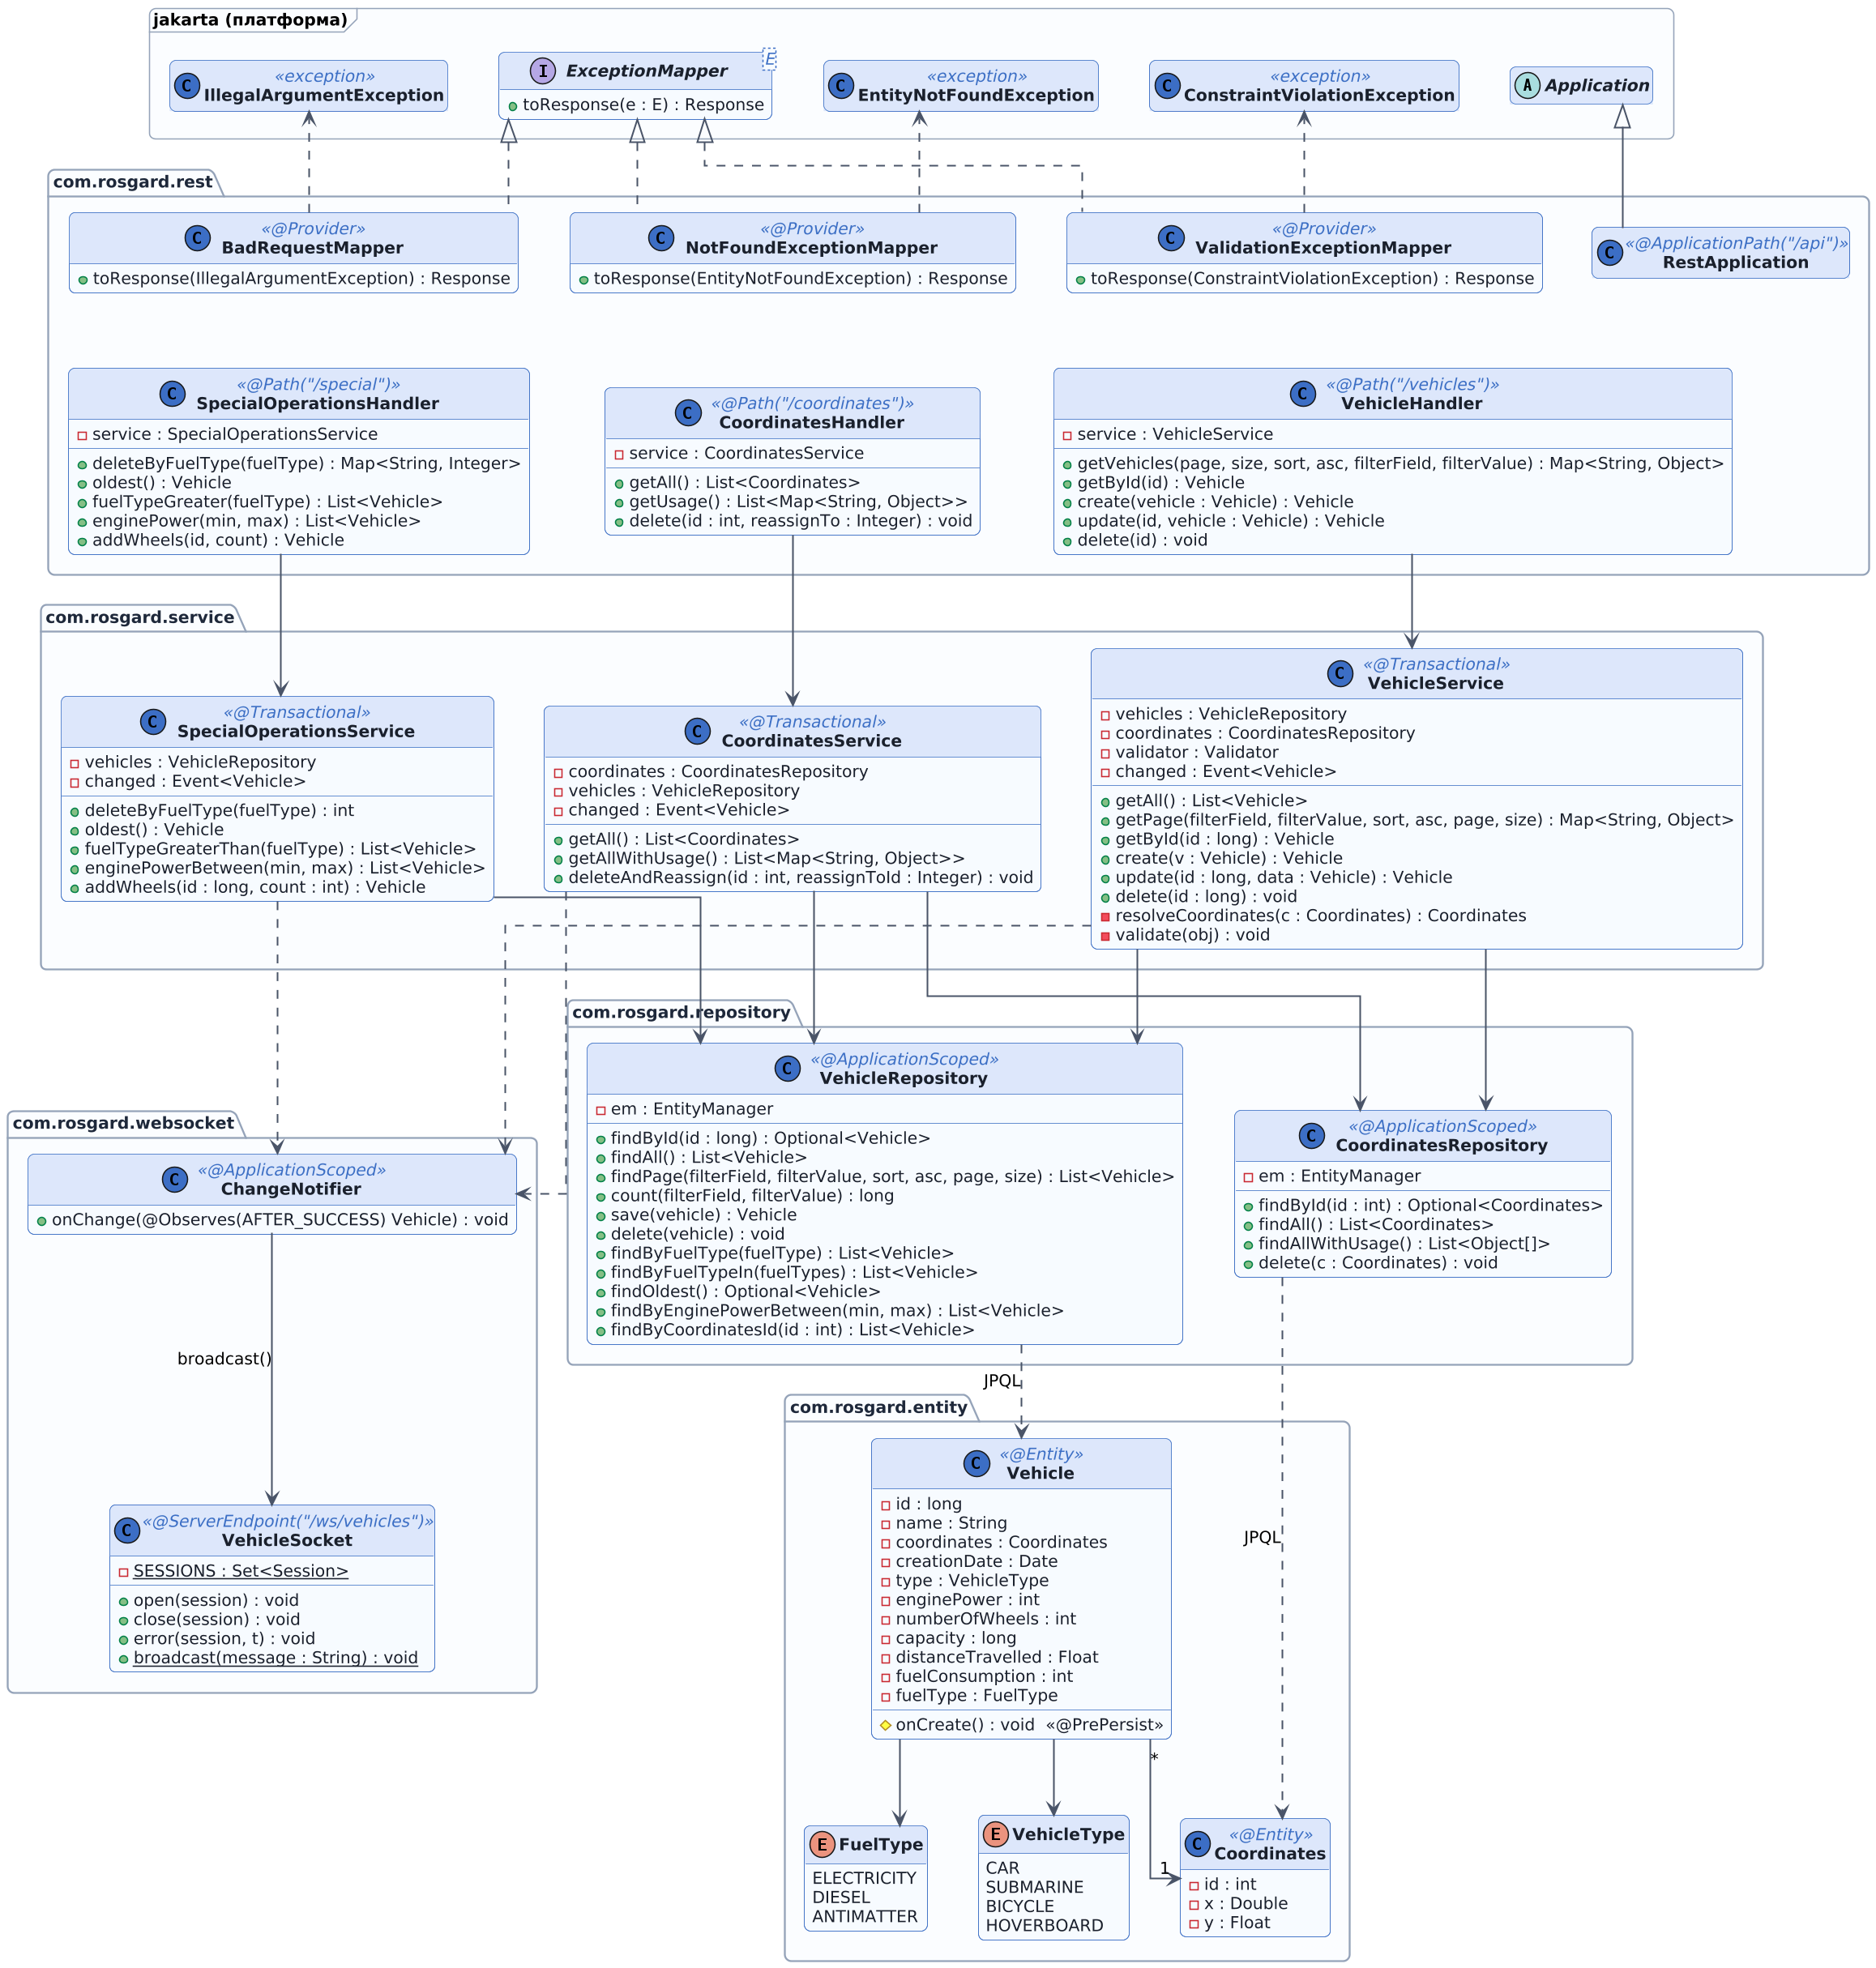
\includegraphics[width=\textwidth,height=0.9\textheight,keepaspectratio]{classes.png}
    \caption{Диаграмма классов}
    \label{fig:classes}
\end{figure}

\newpage
\subsection{Диаграмма пакетов}

Серверный код разделён на пакеты по слоям. Зависимости идут только сверху вниз: \texttt{rest} знает про \texttt{service}, \texttt{service} --- про \texttt{repository}, и все они используют \texttt{entity}. Единственная связь «вбок» --- от \texttt{service} к \texttt{websocket}, и она идёт через CDI-событие, так что сервисы не вызывают WebSocket напрямую. Клиентская часть обращается к серверу двумя путями: запросами к REST API и через WebSocket-соединение.

\begin{figure}[H]
    \centering
    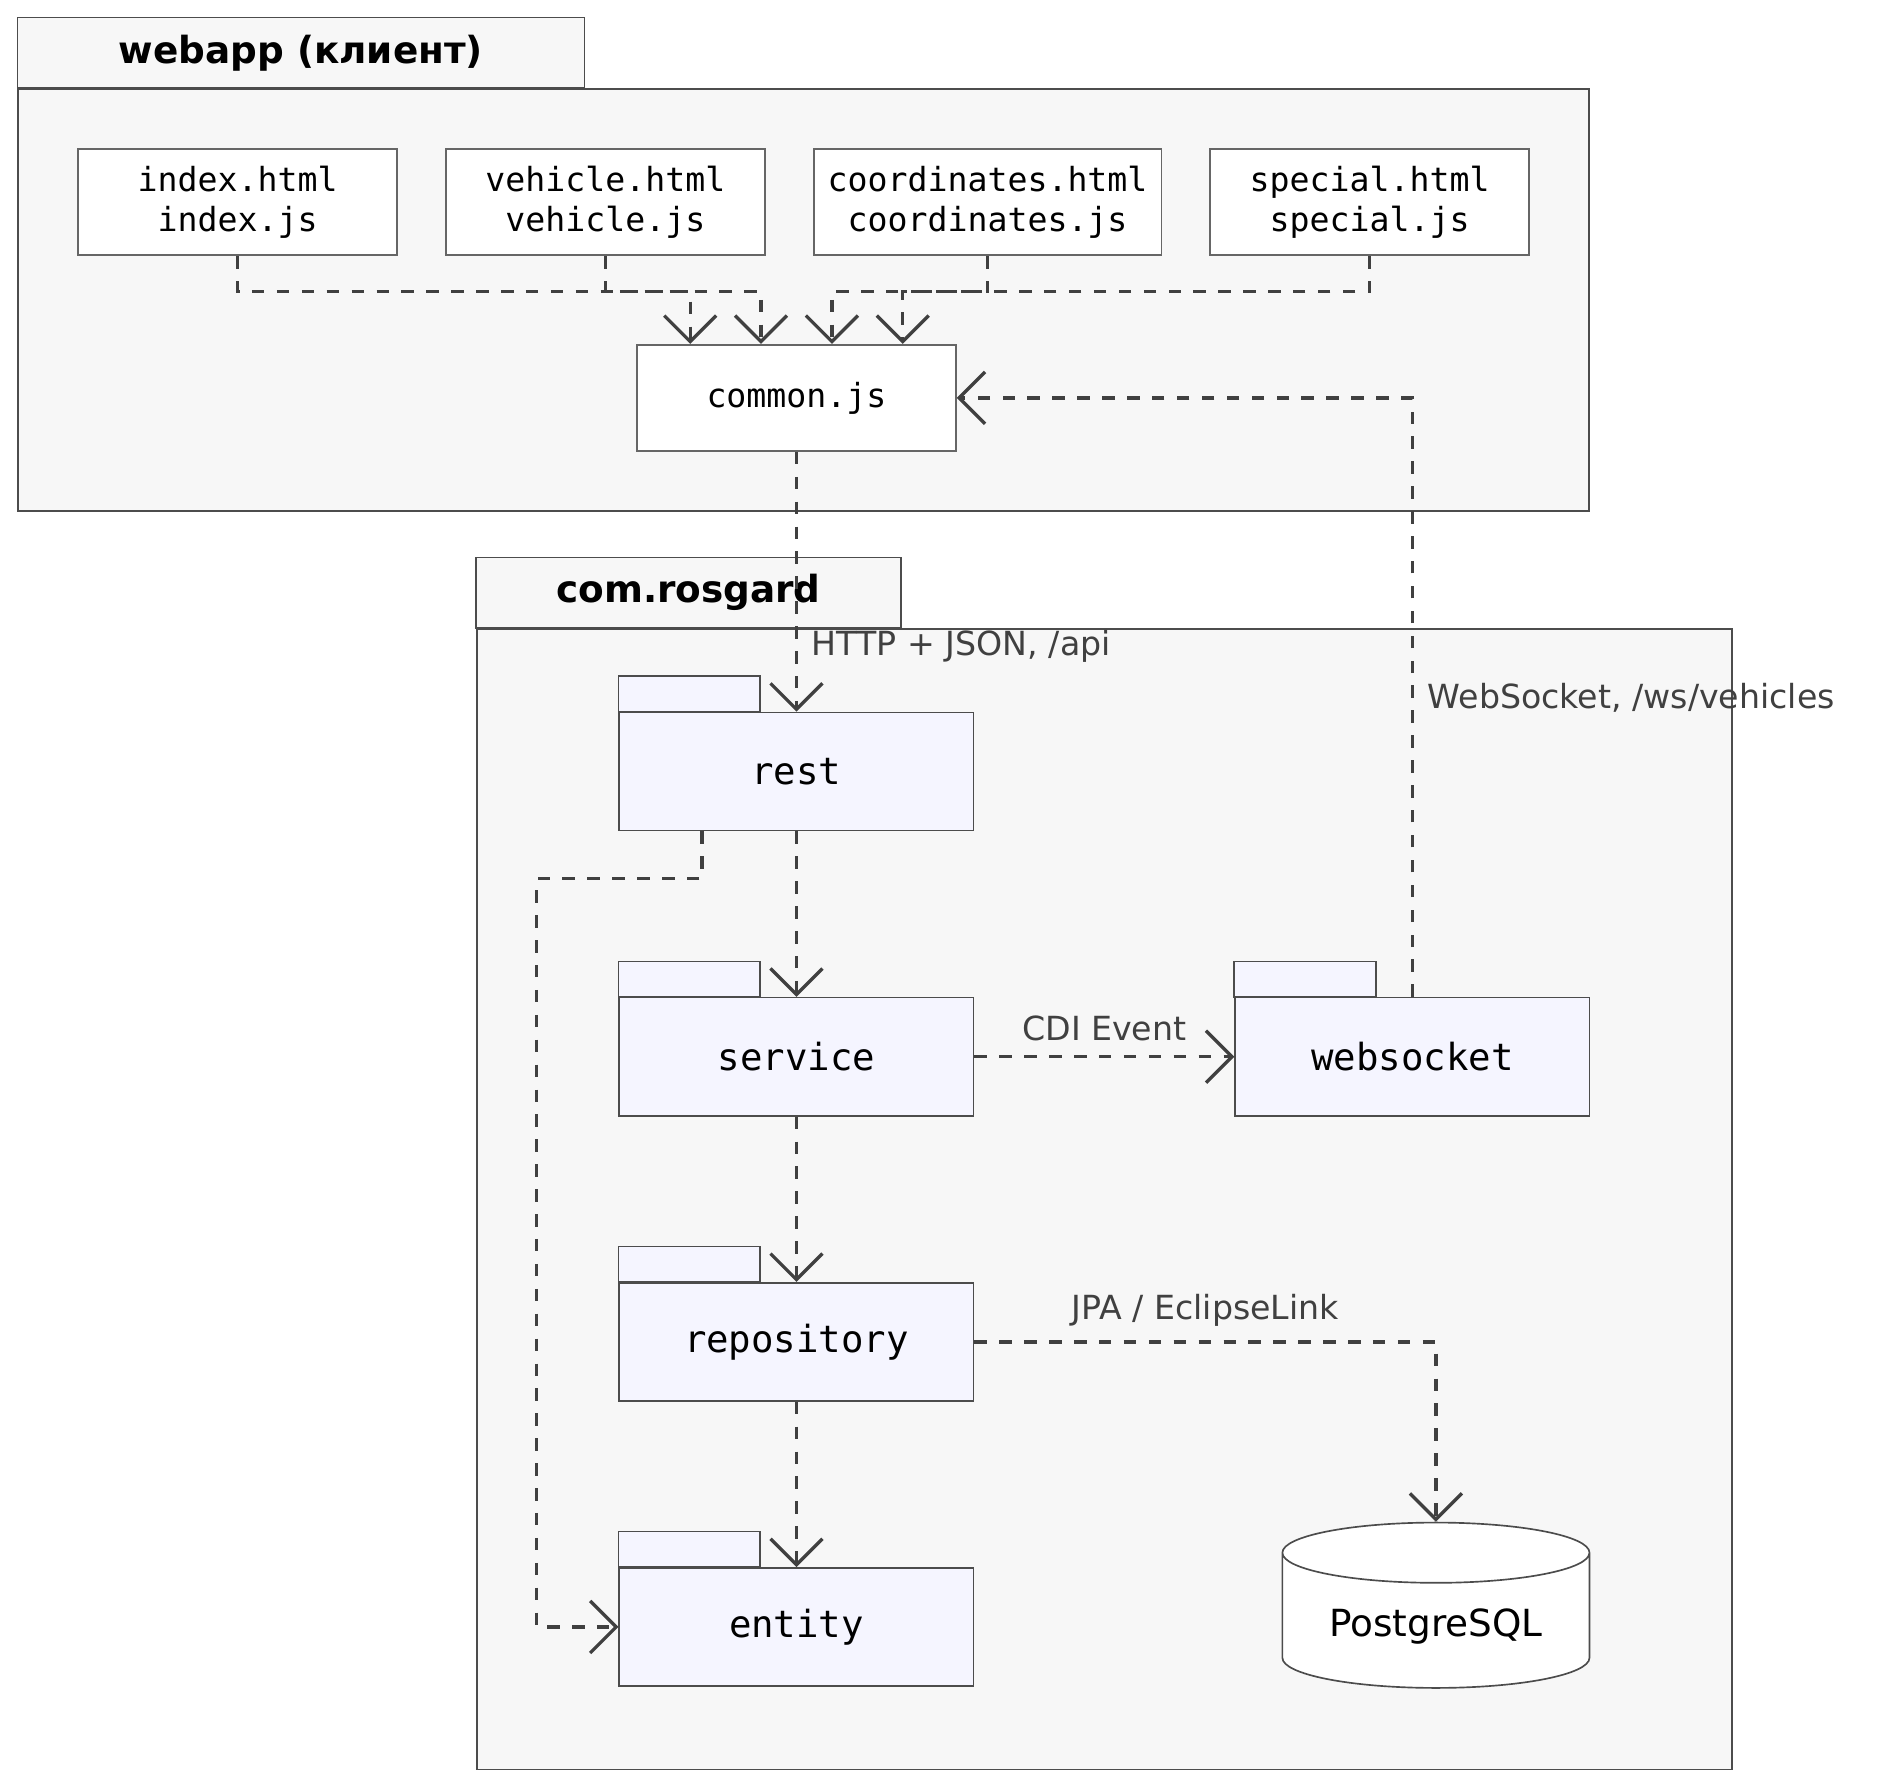
\includegraphics[width=0.92\textwidth]{packages.png}
    \caption{Диаграмма пакетов}
    \label{fig:package-diagram}
\end{figure}

\newpage
\section{Исходный код}

Исходный код лежит в репозитории \url{https://github.com/RosgardX/itmo-labs}, в каталоге \texttt{IS/IS1}. Код я выкладывал не одним коммитом, а цепочкой pull request'ов по слоям: модель, репозитории, сервисы, WebSocket, REST, интерфейс и отчёт. Каждая ветка создана от предыдущей, поэтому в каждом PR видно только то, что добавляет этот слой, и его можно проверить отдельно.

\section{Описание решения}

\subsection{Архитектура}

Приложение я разделил на слои, каждый в своём пакете:

\begin{itemize}[leftmargin=1.2cm]
    \item \texttt{entity} --- классы предметной области, размеченные аннотациями JPA;
    \item \texttt{repository} --- работа с базой через \texttt{EntityManager} и JPQL, больше ничего;
    \item \texttt{service} --- бизнес-логика: проверки, транзакции, спецоперации;
    \item \texttt{rest} --- тонкий слой, который принимает HTTP-запрос, вызывает сервис и отдаёт JSON;
    \item \texttt{websocket} --- оповещение клиентов об изменениях.
\end{itemize}

Так у каждого класса одна задача. REST-ресурсы ничего не знают о базе, а репозитории --- о HTTP. Если завтра понадобится, например, вызывать те же операции не из REST, а из другого места, сервисы можно переиспользовать без изменений. Все компоненты --- CDI-бины с областью \texttt{@ApplicationScoped}, связи между ними задаются через \texttt{@Inject}.

\subsection{Хранение и ограничения полей}

По заданию все ограничения полей должны выполняться и на уровне ORM, и на уровне БД. Я сделал оба уровня явно. На стороне Java стоят аннотации Bean Validation (\texttt{@NotNull}, \texttt{@NotBlank}, \texttt{@Positive} и другие) с понятными сообщениями на русском. На стороне базы каждое поле описано через \texttt{columnDefinition} с \texttt{NOT NULL} и \texttt{CHECK}, например \texttt{integer NOT NULL CHECK (enginePower > 0)}.

Зачем два уровня: проверка в Java даёт пользователю нормальное сообщение об ошибке ещё до обращения к базе, а \texttt{CHECK} в базе гарантирует, что некорректная строка не попадёт в таблицу, даже если её вставят в обход приложения.

Идентификатор генерирует сама база: \texttt{@GeneratedValue(strategy = IDENTITY)} и тип \texttt{bigserial}. Дата создания проставляется автоматически в методе с \texttt{@PrePersist}, так что клиент не может её подменить.

Координаты я вынес в отдельную сущность \texttt{Coordinates} со связью \texttt{@ManyToOne}. Это нужно для требования «связать новый объект с уже существующими вспомогательными объектами»: несколько машин могут ссылаться на одни координаты, и при создании можно выбрать уже существующие координаты, а не вводить их заново.

Схему таблиц создаёт EclipseLink при деплое (\texttt{schema-generation} со значением \texttt{create}). Я выбрал \texttt{create}, а не \texttt{drop-and-create}, чтобы данные не стирались при каждом передеплое.

\subsection{Валидация и сообщения об ошибках}

Все проверки выполняются на сервере, в сервисах. Перед сохранением сервис вызывает \texttt{Validator}, и если есть нарушения, бросает \texttt{ConstraintViolationException}. Для случаев «объект не найден» и «неверный параметр» сервисы бросают \texttt{EntityNotFoundException} и \texttt{IllegalArgumentException}.

Превращать исключения в HTTP-ответы я поручил мапперам JAX-RS. Их три, по одному на тип ошибки, и каждый возвращает ответ с кодом 400 или 404 и телом вида \texttt{\{"errors": [...]\}}. Благодаря этому в REST-ресурсах нет ни одного \texttt{try/catch}, а клиент всегда получает ошибки в одном формате и просто выводит их список под формой.

На клиенте тоже есть ограничения ввода (\texttt{required}, \texttt{min}, \texttt{max} у полей формы), но это только для удобства: сервер всё равно проверяет данные сам.

\subsection{Таблица: пагинация, фильтрация и сортировка}

Пагинацию, фильтрацию и сортировку я сделал на сервере, а не в браузере. Если отдавать клиенту всю таблицу и листать её на месте, то при большом числе объектов страница будет грузиться всё дольше. Сервер же возвращает только нужную страницу (через \texttt{setFirstResult} и \texttt{setMaxResults}) и общее число найденных записей, чтобы клиент мог нарисовать номера страниц.

Фильтрация работает по неполному совпадению: по названию через \texttt{LOWER(name) LIKE}, по типу и типу топлива --- по совпадению части названия значения перечисления.

Отдельно пришлось подумать о сортировке. Поле сортировки приходит от клиента строкой и подставляется в текст JPQL-запроса, а параметром запроса его передать нельзя. Чтобы через это поле нельзя было внедрить произвольный JPQL, я храню список разрешённых полей и отклоняю всё остальное:

\begin{code}
if (!SORT_FIELDS.contains(sort)) throw new IllegalArgumentException("Нельзя сортировать по полю " + sort);
\end{code}

\subsection{Удаление координат с перепривязкой}

Если удалить координаты, на которые ссылаются машины, внешний ключ в базе не даст это сделать. По заданию пользователь должен выбрать, к каким другим координатам привязать эти машины. Поэтому на странице координат рядом с каждой записью показывается, сколько машин к ней привязано, а при удалении появляется выбор новых координат.

На сервере всё происходит в одной транзакции: сервис находит привязанные машины, переставляет им ссылку на выбранные координаты и только потом удаляет старые. Если что-то пойдёт не так, транзакция откатится целиком и машины не останутся без координат. Если пользователь не выбрал, куда перепривязать, или выбрал те же координаты, сервер вернёт понятную ошибку.

\subsection{Синхронизация клиентов}

Задание требует, чтобы изменения сразу появлялись у всех пользователей. Я рассматривал несколько вариантов:

\begin{enumerate}[leftmargin=1.2cm]
    \item Short polling --- клиент раз в несколько секунд сам спрашивает сервер, не изменилось ли что-нибудь;
    \item Long polling --- клиент отправляет запрос, а сервер держит его открытым, пока не появятся изменения;
    \item Server-Sent Events --- сервер отправляет события по одному постоянному HTTP-соединению;
    \item WebSocket --- постоянное двустороннее соединение.
\end{enumerate}

Short polling я отбросил сразу: он постоянно нагружает сервер и базу запросами, даже когда ничего не меняется, и всё равно даёт задержку. Long polling --- по сути обходной путь, чтобы получить то же, что дают SSE или WebSocket. Между SSE и WebSocket я выбрал WebSocket: он входит в Jakarta EE (\texttt{jakarta.websocket}) и уже есть в WildFly, сервер на нём пишется одним классом с \texttt{@ServerEndpoint}, а на клиенте хватает стандартного объекта \texttt{WebSocket} без библиотек. То, что WebSocket двусторонний, мне здесь не нужно, но и не мешает.

Важный момент --- когда именно отправлять уведомление. Если отправить его сразу после изменения в сервисе, клиент может перезапросить данные раньше, чем транзакция закоммитится, и получить старое состояние. Поэтому сервисы только публикуют CDI-событие, а \texttt{ChangeNotifier} принимает его с фазой \texttt{AFTER\_SUCCESS}, то есть уже после успешного коммита:

\begin{code}
public void onChange(@Observes(during =                   TransactionPhase.AFTER_SUCCESS) Vehicle changed) {
    VehicleSocket.broadcast("vehicles");
}
\end{code}

Заодно так сервисы не зависят от WebSocket напрямую: они не знают, кто слушает событие.

В сообщении я передаю не сам изменённый объект, а только сигнал «данные изменились». У каждого пользователя своя страница таблицы, свой фильтр и своя сортировка, и по одному объекту клиент не может понять, попадает ли он на его страницу и куда. Проще и надёжнее при сигнале перезапросить текущую страницу с теми же параметрами. Если соединение оборвалось, клиент через пару секунд подключается заново.

\subsection{Специальные операции}

Все пять операций находятся в отдельном сервисе
\texttt{Special\-Operations\-Service}, а вызываются они с отдельной страницы. По заданию их нельзя делать функциями и процедурами БД, поэтому логика написана на Java, а к базе идут только обычные JPQL-запросы через репозиторий:

\begin{itemize}[leftmargin=1.2cm]
    \item удаление по типу топлива: сервис находит все такие машины и удаляет их, а клиенту возвращает, сколько удалено;
    \item объект с минимальной датой создания: запрос с сортировкой по \texttt{creationDate} и ограничением в одну запись;
    \item объекты с типом топлива больше заданного: «больше» я понимаю как порядок значений в перечислении \texttt{FuelType}. Сервис сам вычисляет, какие значения идут после заданного, и ищет машины с любым из них;
    \item поиск по диапазону мощности: запрос с \texttt{BETWEEN}, а если минимум больше максимума, сервер возвращает ошибку;
    \item добавление колёс: сервис находит машину, проверяет, что число колёс положительное и сумма не переполнит \texttt{int}, и меняет поле. Отдельный \texttt{save} не нужен: объект управляется \texttt{EntityManager}, и изменение запишется в базу при коммите транзакции.
\end{itemize}

Операции, которые меняют данные, тоже публикуют событие, так что результат сразу виден у всех клиентов.

\subsection{Клиентская часть}

Интерфейс я написал на обычных HTML, CSS и JavaScript, без фреймворков. Страниц всего четыре, и сборщик или отдельный фреймворк для них был бы лишним. Все данные клиент получает от REST API и сам строит таблицу.

Общий код вынесен в \texttt{common.js}: меню для перехода между разделами (объекты, координаты, спецоперации), диалог создания и редактирования, вывод ошибок и подключение к WebSocket. Создание и редактирование открываются в отдельном диалоговом окне, причём редактировать можно и из таблицы, и со страницы просмотра объекта. В форме можно выбрать уже существующие координаты или ввести новые.

\subsection{Сборка и развёртывание}

Проект собирается Maven в \texttt{IS1.war}. Используются Java 17, Jakarta EE API 11 и EclipseLink 4.0.4. Для EclipseLink я подключил только модуль JPA (\texttt{org.eclipse.persistence.jpa}): полный артефакт тянет за собой MOXy, который подменял сериализацию JSON и ломал ответы с \texttt{Map} и \texttt{List}.

Приложение не содержит параметров подключения к базе: в \texttt{persistence.xml} указан только JNDI-ресурс \texttt{java:\allowbreak jboss/\allowbreak datasources/\allowbreak IS1}. Во время разработки я запускал его на локальном WildFly с локальной базой PostgreSQL, а для сдачи настроил такой же datasource на WildFly на сервере helios, подключённый к базе \texttt{studs} на хосте \texttt{pg}. Код приложения при этом менять не пришлось.

\newpage
\section{Выводы}

В ходе работы я разработал информационную систему для управления объектами \texttt{Vehicle} на Jakarta EE. Приложение разделено на слои: сущности, репозитории, сервисы, REST API и WebSocket, и у каждого слоя своя ответственность.

Ограничения полей выполняются и на уровне ORM через Bean Validation, и на уровне базы через \texttt{NOT NULL} и \texttt{CHECK}. Ошибки обрабатываются централизованно мапперами JAX-RS и доходят до пользователя понятными сообщениями. Таблица поддерживает серверную пагинацию, фильтрацию и сортировку, а изменения сразу появляются у всех клиентов благодаря WebSocket и CDI-событиям, которые срабатывают после коммита транзакции.

Я разобрался, как устроены JPA и EclipseLink, как CDI связывает компоненты и доставляет события, как JAX-RS сам вызывает мапперы исключений и почему уведомлять клиентов нужно только после коммита.

\end{document}
